\section{Entanglement generation}\label{sec:4:entanglement-generation}
The averaged state $\mean{\rho}$ after multiple measurements is given by
\begin{equation}\label{eq:4:average-density}
  \mean{\rho} = \int_{-\infty}^{\infty} \dd \theta_A p(\theta_A) \int_{-\infty}^{\infty} \dd \theta_B p(\theta_B) \int_{-\infty}^{\infty} \dd L_A p(L_A) \int_{-\infty}^{\infty} \dd L_B p(L_B) \ \rho(\theta_A, \theta_B, L_A, L_B)
\end{equation} 
where $p(\,\cdot\,)$ represents the Gaussian distributions of the random variables 
$\theta_{A(B)}$ and $L_{A(B)}$ with standard deviations $\Delta \theta$ or $\Delta L$ respectively. 
$\rho(\theta_A, \theta_B, L_A, L_B)$ denotes the state of the system on a given experimental run where the parameters for the initial placement take the values $\theta_A$, $\theta_B$, $L_A$ and $L_B$. 
The state $\rho_0$ at $t=0$ is given as before by eq. \eqref{eq:2:initial-state}.
Beyond mutual gravitational interactions, the dynamic phases $\phi^{(i)}_{A(B),\,\mathrm{Cas}}(t)$ are induced on the cat-states $\ket{\psi^{(i)}_{A(B)}}$ ($i = 1, 2$) by Casimir interactions with the Faraday shield.
Using the two different models for the Casimir attraction for large and small separations given by eq. \eqref{eq:3:casimir-sphere-plate-PFA} and eq. \eqref{eq:3:casimir-sphere-plate-PFA}, it follows
\begin{equation}
  \phi^{(i)}_{A(B),\,\mathrm{Cas}}(t) = \frac{t}{\hbar}
  \begin{cases}
     \frac{3 \hbar c}{8 \pi} \left(\frac{\varepsilon_r - 1}{\varepsilon_r + 2}\right) \frac{R^3}{\left(L^{(i)}_{A(B)}\right)^4} & \text{for large separations (LSL)} \\
    \frac{\hbar c \pi^3}{720} \varphi(\varepsilon_r) \left(\frac{\varepsilon_r - 1}{\varepsilon_r + 1}\right) \frac{R}{\left(\mathscr{L}^{(i)}_{A(B)}\right)^2} & \text{for small separations (PFA) .}
  \end{cases}
\end{equation}
Here, $L^{(i)}_{A(B)}$ and $\mathscr{L}^{(i)}_{A(B)} = L^{(i)}_{A(B)}-R$ are the distances between the particles and the shield's surface given by
\begin{align}\label{eq:4:L-casimir}
  L^{(i)}_{A} &= L + L_{A} - \frac{d}{2} \pm_i \frac{\Delta x_{A}}{2} \sin(\alpha + \theta_{A}) \quad \quad \text{and} \\
  L^{(i)}_{B} &= L + L_{B} - \frac{d}{2} \mp_i \frac{\Delta x_{B}}{2} \sin(\beta + \theta_{B})
\end{align}
where $\pm_i = -(-1)^{i}$ distinct between the two components that conform the cat-state of a single particle.
The gravitationally induced phase between states $\ket{\psi^{(i)}_A}\otimes\ket{\psi^{(j)}_B}$ is given analogue to the previous calculations in \cref{cha:first-look} as
\begin{equation}\label{eq:4:phi-grav}
  \phi^{(ij)}_\mathrm{Grav}(t) = \frac{t}{\hbar} \frac{G M_A M_B}{L^{(ij)}} .
\end{equation}
The separation $L^{(ij)}$ between the particle cat-states $A^{(i)}$ and $B^{(j)}$ is given by
\begin{multline}\label{eq:4:L-gravity}
  L^{(ij)} = \sqrt{\left(2L + L_A + L_B \pm_i \frac{\Delta x_A}{2}\sin(\alpha + \theta_A) \mp_j \frac{\Delta x_B}{2}\sin(\beta + \theta_B)\right)^2 +} \\ \overline{\left(\frac{\Delta x_A}{2}\cos(\alpha + \theta_A) \mp_{i=j} \frac{\Delta x_B}{2}\cos(\beta + \theta_B)\right)^2}
\end{multline}
with $\mp_{i=j} = +(-1)^{\delta_{ij}}$.
Expanding to first order in $\Delta x_{A(B)} \ll L$, $\theta_{A(B)} \ll 1$ and $L_{A(B)} \ll L$ (which is justified as seen in the following), the averaged evolved state 
$\mean{\rho}$ in eq. \eqref{eq:4:average-density} is analytically obtainable, as shown in \cref{apx:placement-average-density-matrix}.
Assuming $\Delta \theta_A = \Delta \theta_B \equiv \Delta\theta$ and $\Delta L_A = \Delta L_B \equiv \Delta L$, the off-diagonal elements (the so-called \textit{coherences}) decay with
\begin{equation}\label{eq:4:average-density-element}
  \mean{\rho_{kl}} = \frac{1}{4} e^{i \Delta \phi_{kl}(t)} \exp{-\frac{(\xi_{kl})^2}{2} (\Delta\theta)^2 t^2} \exp{-\frac{(\zeta_{kl})^2}{2} (\Delta L)^2 t^2}
\end{equation}
where $\Delta \phi$, $\xi$ and $\zeta$ are substitutes for lengthy expressions given by eq. \eqref{eq:apx:phi-definition}, eq. \eqref{eq:apx:definition-xi} and eq. \eqref{eq:apx:definition-zeta} in the appendix and are dependent on system parameters.
For $\Delta \theta, \Delta L \rightarrow \infty$ or $t\rightarrow \infty$, coherences vanish, resulting in a maximally mixed state with $\tr\rho^2 = 1/4$ - which is not entangled.
For sufficiently large variations in the initial placement of the particles, one expects the loss of entanglement even at arbitrarily short times.
\begin{table}[!t]
  \centering
  \begin{adjustbox}{max width=\textwidth}
    \begin{tabularx}{\textwidth}{c c c c c c c}
      \toprule
      \multirow{2}{*}{Orientation} & \multicolumn{2}{c}{Particle size} & \multirow{2}{*}{$L$} & \multirow{2}{*}{$\Delta x$} & \multicolumn{2}{c}{Shield size $^b$} \\ \cline{2-3} \cline{6-7}
      & Radius $R$ & Mass $M$ $^a$ & & & $d$ & $r_s$\\
      \midrule
      \begin{tabular}{@{}c@{}}Parallel \\ ($\alpha=\beta=0$) \end{tabular} & \begin{tabular}{@{}c@{}}$10\si{\mu m}$ \\ $=10^{-5}\si{m}$\end{tabular} & \begin{tabular}{@{}c@{}}$\approx 10^{-11}\si{kg}$ \\ $=5\times 10^{-4} \, m_p$\end{tabular} & $2R=20\si{\mu m}$ & $100\si{nm}$ & $100\si{nm}$ & $1\si{cm}$ \\
      \bottomrule
      \multicolumn{7}{l}{\footnotesize $^a$ Here $m_p = \sqrt{c\hbar/G}\approx 2.17\times 10^{-8}\si{kg}$ is the Planck mass. $^b$ The required size of the shield is later} \\[-4pt]
      \multicolumn{7}{l}{\footnotesize estimated in section 5.1.} \\[5pt]
    \end{tabularx}
  \end{adjustbox}
  \caption{Default parameters for the setup in \cref{fig:4:complete-setup}. Maximum entanglement is reached after $t_\mathrm{max} = 258\si{ms}$ for these parameters. They were chosen in accordance with multiple proposals \cite{Aspelmeyer_2024,Rijavec_2021}. Both particles are assumed to be identical. The thickness $d$ and radius $r_s$ of the shield is estimated in \cref{sec:5:shield-size}.}
  \label{tab:paramters}
\end{table}

For the special case of two identical particles and $\alpha=\pm\beta$, the logarithmic negativity $E_N$ is approximated to first order as
\begin{equation}\label{eq:4:log-neg-analytical}
  E_N(\mean{\rho}) = \max\left\{ 0,\ \log_2\left(e^{-\gamma}\left(\cosh\gamma + \abs{\sin \phi}\right)\right) \right\}
\end{equation}
where the decoherence parameter $\gamma = \left(\xi^2(\Delta \theta)^2/2 + \zeta^2(\Delta L)^2/2\right)t^2$ is given in eq. \eqref{eq:apx:stochastic-decoherence} and the phase $\phi$ is given by eq. \eqref{eq:4:phi-orientation} in the next section.
Numerical results validate this approximation and are shown in \cref{fig:4:EN-variations} for varying $\Delta \theta$ and $\Delta L$ in the parallel configuration.
\begin{figure}[!htb]
  \centering
  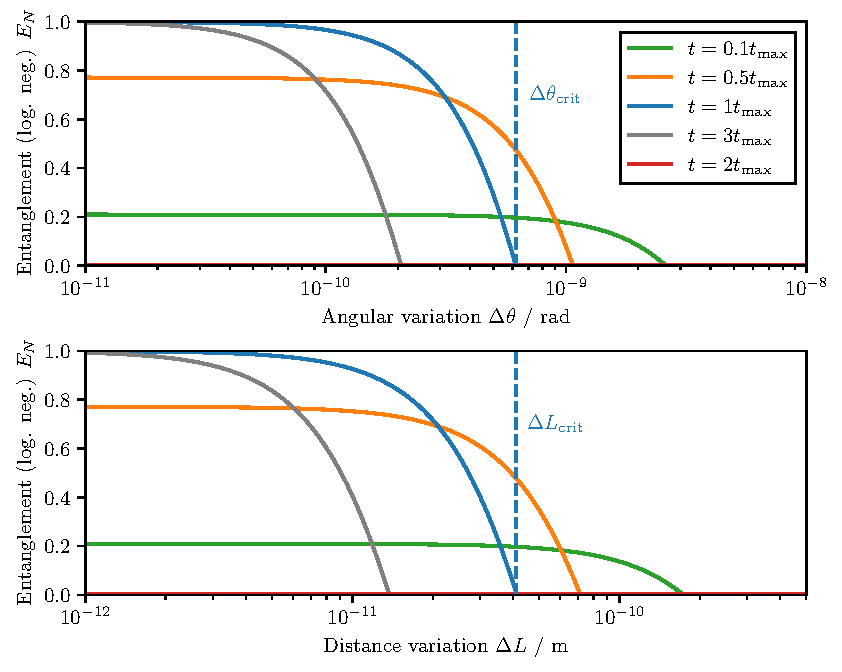
\includegraphics[width=\textwidth]{./../figures/theta-variance/EN-deltaTheta-deltaL.pdf}
  \caption{Entanglement quantified by the logarithmic negativity dependent on the placement variations in the initial setup $\Delta \theta$ and $\Delta L$. The entanglement is shown at different times, where $t_\mathrm{max} \approx 258\si{ms}$ is the time from eq. \eqref{eq:4:t-max}, after which maximal entanglement is reached. At a critical point $\Delta \theta_\mathrm{crit}$ or $\Delta L_\mathrm{crit}$, all entanglement is lost. The used parameters are taken from \cref{tab:paramters}.}
  \label{fig:4:EN-variations}
\end{figure}
For small placement variations, the system remains entangled.
However, once the critical thresholds $\Delta \theta_\mathrm{crit}$ and $\Delta L_\mathrm{crit}$ are surpassed, entanglement is lost entirely.
The critical decoherence threshold $\gamma_\mathrm{crit}$ is given by
\begin{equation}\label{eq:4:critical-point}
  \gamma_\mathrm{crit} = \log(1 + \sqrt{2}) = \mathrm{const.}
\end{equation}
which imposes $\Delta\theta_\mathrm{crit} \propto 1/(\xi t)$ and $\Delta L_\mathrm{crit} \propto 1/(\zeta t)$. 
For the parameters in \cref{tab:paramters}, these thresholds are around $\Delta \theta_\mathrm{crit} \approx 6 \times 10^{-10} \si{rad}$ and $\Delta L_\mathrm{crit} \approx 1.4 \times 10^{-10} \si{m}$, which seems challenging experimentally.
For all these calculations, the radius of the particles is set to $R=10^{-5}\si{m} = 10\si{\mu m}$ with corresponding masses $M=4/3 \pi R^3 \rho_\mathrm{Silica} \approx 1.1\times 10^{-11}\si{kg}$.
A particle-shield separation of $L=2R$ and a superposition size of $\Delta x = 100\si{nm}$ are used.
In the rest of this thesis, if not otherwise specified, these parameters are used as a default.
For convenient retrieval, they are collectively displayed in \cref{tab:paramters} at the top of the previous page.

These values are consistent with theoretical proposals (see e.g. the Tab. 1 in Ref. \cite{Rijavec_2021}) as they result in a low one-run duration of $t_\mathrm{max}\approx 258\si{ms}$ \cite[Timestamp: 51:00]{Aspelmeyer_2024}, but remain beyond current experimental capabilities.
The largest mass demonstrated in matter-wave interferometry is around $4\times 10^{-23}\si{kg}$ \cite{Fein_2019} with a spatial superposition size of $\Delta x \gtrsim 500\si{nm}$.
In solid-state opto-mechanical systems, quantum control and ground-state cooling have been demonstrated with masses of $10^{-13}\si{kg}$ with mechanical oscillators coupled to superconducting qubits \cite{OConnell_2010}; entangled diamonds with $10^{-11}\si{kg}$ have been observed \cite{Lee_2011} and masses of $10^{-8}\si{kg}$ have been prepared in motional center-of-mass cat-states \cite{Bild_2023}, although with short coherence times $\ll 1\si{\mu s}$.
Also impressive and notable is the cooling of the differential oscillation mode between the four $\sim 40\si{kg}$ LIGO mirrors to only very few occupied phonon states \cite{Whittle_2021}.
In contrast, the smallest mass with a measurable gravitational force is around $92 \si{mg}$ \cite{Westphal_2021}.
The field of levitated nano-particles has the potential to bridge thw worlds of molecular superposition and mechanical systems, offering exceptional quantum control, high force sensitivity and long coherence times up to seconds \cite{Aspelmeyer_2024}.
Thus many proposals aim to measure quantum entanglement due to gravity between trapped and levitated particles \cite{Krisnanda_2020,GonzalezBallestero_2021}.

Nonetheless, the required accuracy in the placement of the particles appears very challenging experimentally.
However, looking at the entanglement dynamics in \cref{fig:4:EN-dynamics-variations}, for shorter times $t<t_\mathrm{max}$, greater variations in particle placement can be tolerated at the cost of reduced entanglement and thus requiring a greater precision in the actual measurement process.
\begin{figure}[!htbp]
  \centering
  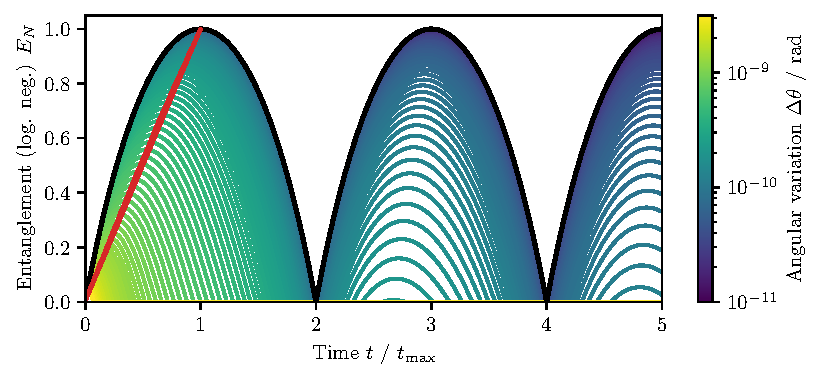
\includegraphics[width=\textwidth]{./../figures/theta-variance/EN-dynamics-delta-theta.pdf}
  \caption{Entanglement dynamics after eq. \eqref{eq:4:log-neg-analytical} for different angular variations $\Delta \theta$ for the parameters used in \cref{tab:paramters}. The black outer most line shows the ideal case without any placement variations and aligns with \cref{fig:2:entanglement-dynamics}. For large variations, entanglement is only observable during a brief window of time with an optimal measurement time colored in red.}
  \label{fig:4:EN-dynamics-variations}
\end{figure}
At these shorter times, the gravitational interaction has not fully entangled the particles, and decoherence (which scales as $\gamma \propto t^2$) has not yet significantly developed.
If achieving the maximum entanglement is not required and \textit{any} amount of entanglement $E_N > 0$ suffices, it may be advantageous to perform measurements at $t < t_\mathrm{max}$.
This, of course, requires ensuring that other entanglement mechanisms contribute smaller entanglement rates (see \cref{cha:the-shield} for further discussion).
Decoherence effects from collisions with air molecules, thermal black-body radiation, fluctuations in the trapping fields, external vibrations and unwanted interactions with stray fields (including gravitational fields from nearby non-stationary objects) should also be taken into account.
The optimal measurement time for a required level of entanglement is depicted in \cref{fig:4:time-delta-theta}.
\begin{figure}[!htbp]
  \centering
  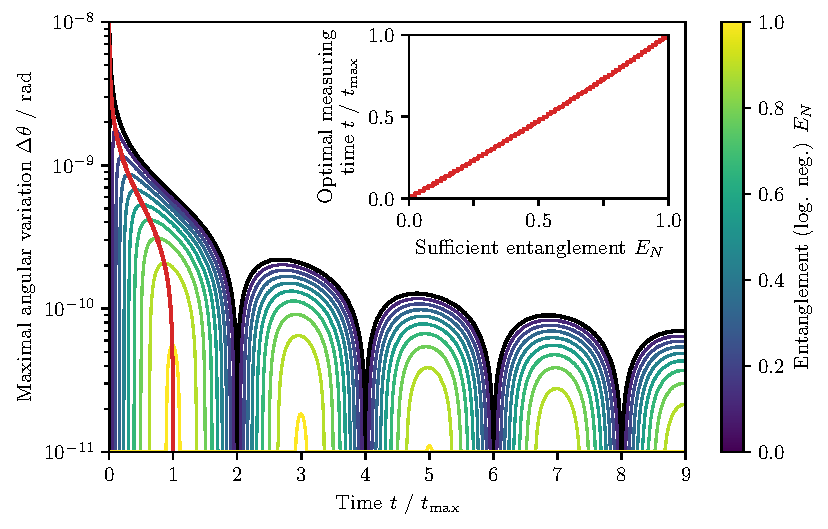
\includegraphics[width=\textwidth]{./../figures/theta-variance/time-delta-theta-crit-EN.pdf}
  \caption{Contour plot of the maximal angular variation for given times after which a specific amount of entanglement $E_N$ is still measurable. The setup parameters are taken from \cref{tab:paramters}. The outer most black line corresponds to the time dependence of $\Delta \theta_\mathrm{crit}$. A fully entangled state with $E_N=1$ is only measurable at $t=t_\mathrm{max}$ with a maximally possible angular variation of around $10^{-11}\si{rad}$. The red curve on the top right shows the optimal measuring time for a specific amount of entanglement and aligns precisely with the red curve in \cref{fig:4:EN-dynamics-variations}. Correspondingly, the red curve in the main figure shows the maximal angular variation for which this goal is reachable. At times $2k t_\mathrm{max},\,k\in\mathbb{N}$ no entanglement can be measured.}
  \label{fig:4:time-delta-theta}
\end{figure}
The figure also provides the corresponding maximum allowable variation for a given time. Conversely, for fixed variations, the optimal measurement time and maximum attainable entanglement can be determined.
It can be seen that at times $2k t_\mathrm{max}, \ k\in\mathbb{N}$ no entanglement is measurable, coinciding with the findings for the ideal scenario in \cref{cha:first-look}. 
